%%
%% Automatically generated file from DocOnce source
%% (https://github.com/doconce/doconce/)
%% doconce format latex movies.do.txt --latex_movie=media9
%%


%-------------------- begin preamble ----------------------

\documentclass[%
oneside,                 % oneside: electronic viewing, twoside: printing
final,                   % draft: marks overfull hboxes, figures with paths
10pt]{article}

\listfiles               %  print all files needed to compile this document

\usepackage{relsize,makeidx,color,setspace,amsmath,amsfonts,amssymb}
\usepackage[table]{xcolor}
\usepackage{bm,ltablex,microtype}

\usepackage[pdftex]{graphicx}

\usepackage{fancybox}  % make sure fancybox is loaded before fancyvrb
%\setlength{\fboxsep}{8pt}  % may clash with need in pre/cod envirs

% Movies are handled by the media9 package
\newenvironment{doconce:movie}{}{}
\newcounter{doconce:movie:counter}
\usepackage{media9}
\usepackage{movie15}
\usepackage{animate}


\usepackage{fancyvrb} % packages needed for verbatim environments
\usepackage{fancyvrb}

\usepackage[T1]{fontenc}
%\usepackage[latin1]{inputenc}
\usepackage{ucs}
\usepackage[utf8x]{inputenc}

\usepackage{lmodern}         % Latin Modern fonts derived from Computer Modern

% Hyperlinks in PDF:
\definecolor{linkcolor}{rgb}{0,0,0.4}
\usepackage{hyperref}
\hypersetup{
    breaklinks=true,
    colorlinks=true,
    linkcolor=linkcolor,
    urlcolor=linkcolor,
    citecolor=black,
    filecolor=black,
    %filecolor=blue,
    pdfmenubar=true,
    pdftoolbar=true,
    bookmarksdepth=3   % Uncomment (and tweak) for PDF bookmarks with more levels than the TOC
    }
%\hyperbaseurl{}   % hyperlinks are relative to this root

\setcounter{tocdepth}{2}  % levels in table of contents

% prevent orhpans and widows
\clubpenalty = 10000
\widowpenalty = 10000

% --- end of standard preamble for documents ---


% insert custom LaTeX commands...

\raggedbottom
\makeindex
\usepackage[totoc]{idxlayout}   % for index in the toc
\usepackage[nottoc]{tocbibind}  % for references/bibliography in the toc

%-------------------- end preamble ----------------------

\begin{document}

% matching end for #ifdef PREAMBLE

\newcommand{\exercisesection}[1]{\subsection*{#1}}

\input{newcommands_bfmath}
\input{newcommands_replace}

% ------------------- main content ----------------------



% ----------------- title -------------------------

\thispagestyle{empty}

\begin{center}
{\LARGE\bf
\begin{spacing}{1.25}
This is a demo of movies in DocOnce
\end{spacing}
}
\end{center}

% ----------------- author(s) -------------------------

\begin{center}
{\bf HPL${}^{}$} \\ [0mm]
\end{center}

\begin{center}
% List of all institutions:
\end{center}
    
% ----------------- end author(s) -------------------------

% --- begin date ---
\begin{center}
Jan 32, 2100
\end{center}
% --- end date ---

\vspace{1cm}


Here is a movie in WebM format.


\begin{doconce:movie}
\refstepcounter{doconce:movie:counter}
\begin{quote}
% link to external viewer
Movie \arabic{doconce:movie:counter}: 1D wave in WebM. \href{run:../doc/src/manual/mov/wave.webm}{\nolinkurl{../doc/src/manual/mov/wave.webm}}
\end{quote}
\end{doconce:movie}


Here is the same movie in Ogg format:


\begin{doconce:movie}
\refstepcounter{doconce:movie:counter}
\begin{quote}
% link to external viewer
Movie \arabic{doconce:movie:counter}: 1D wave in Ogg. \href{run:../doc/src/manual/mov/wave.ogg}{\nolinkurl{../doc/src/manual/mov/wave.ogg}}
\end{quote}
\end{doconce:movie}


Here is the same movie in MP4 format:


\begin{doconce:movie}
\refstepcounter{doconce:movie:counter}
\begin{center}
% media9 package
\includemedia[
label=docsrcmanualmovwavemp4,
width=0.8\linewidth,
activate=pageopen,         % or onclick or pagevisible
addresource=../doc/src/manual/mov/wave.mp4,  % embed the video in the PDF
flashvars={
source=../doc/src/manual/mov/wave.mp4
&autoPlay=true
&loop=true
&scaleMode=letterbox       % preserve aspect ratio while scaling this video
}]{}{VPlayer.swf}
%\mediabutton[mediacommand=docsrcmanualmovwavemp4:playPause]{\fbox{\strut Play/Pause}}
\end{center}

\begin{center}  % movie caption
Movie \arabic{doconce:movie:counter}: 1D wave in MP4.
\end{center}
\end{doconce:movie}


Here is the same movie in Flash format:


\begin{doconce:movie}
\refstepcounter{doconce:movie:counter}
\begin{center}
% media9 package
\includemedia[
label=docsrcmanualmovwaveflv,
width=0.8\linewidth,
activate=pageopen,         % or onclick or pagevisible
addresource=../doc/src/manual/mov/wave.flv,  % embed the video in the PDF
flashvars={
source=../doc/src/manual/mov/wave.flv
&autoPlay=true
&loop=true
&scaleMode=letterbox       % preserve aspect ratio while scaling this video
}]{}{VPlayer.swf}
%\mediabutton[mediacommand=docsrcmanualmovwaveflv:playPause]{\fbox{\strut Play/Pause}}
\end{center}

\begin{center}  % movie caption
Movie \arabic{doconce:movie:counter}: 1D wave in Flash.
\end{center}
\end{doconce:movie}


And here is a collection of images shown as an animation
(\Verb!frame_*.png!):


\begin{doconce:movie}
\refstepcounter{doconce:movie:counter}
\begin{center}
\begin{animateinline}[controls,loop]{1} % frames: ../doc/src/manual/mov/wave_frames/frame_0080.png -> ../doc/src/manual/mov/wave_frames/frame_0129.png
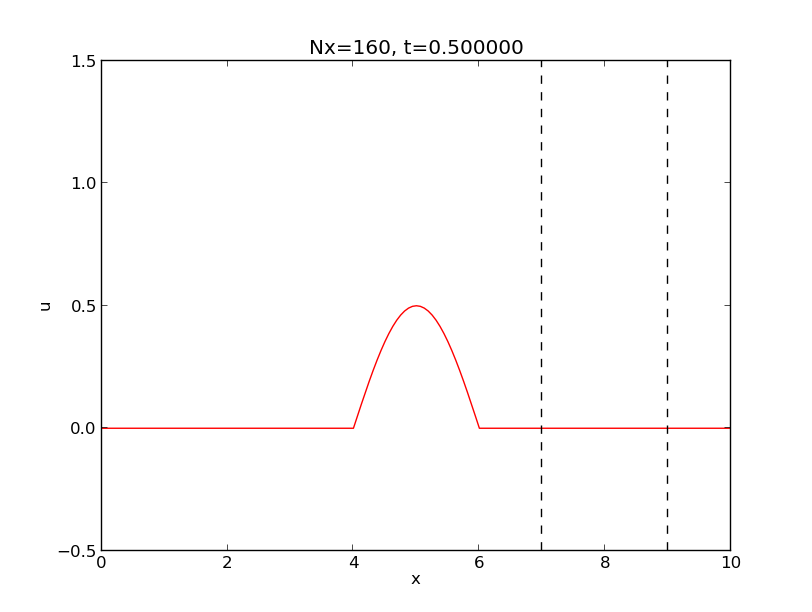
\includegraphics[width=0.9\textwidth]{../doc/src/manual/mov/wave_frames/frame_0080.png}
\newframe
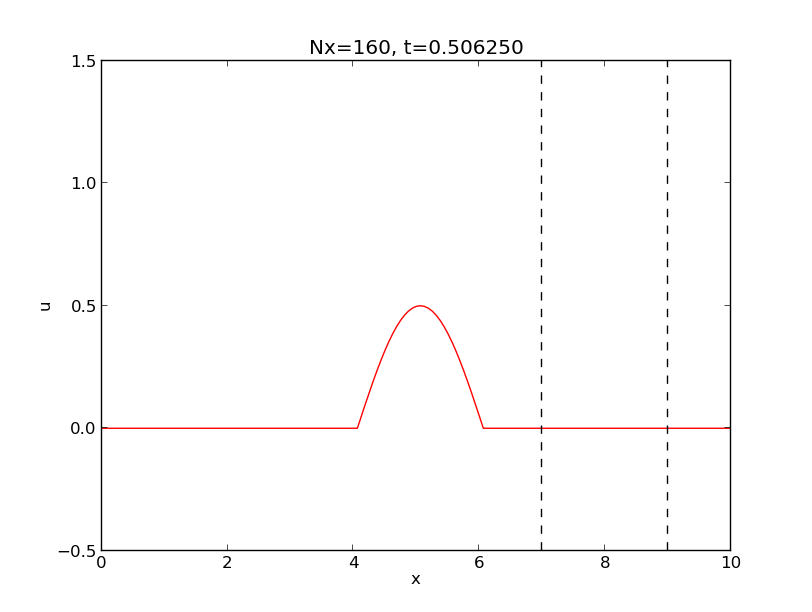
\includegraphics[width=0.9\textwidth]{../doc/src/manual/mov/wave_frames/frame_0081.png}
\newframe
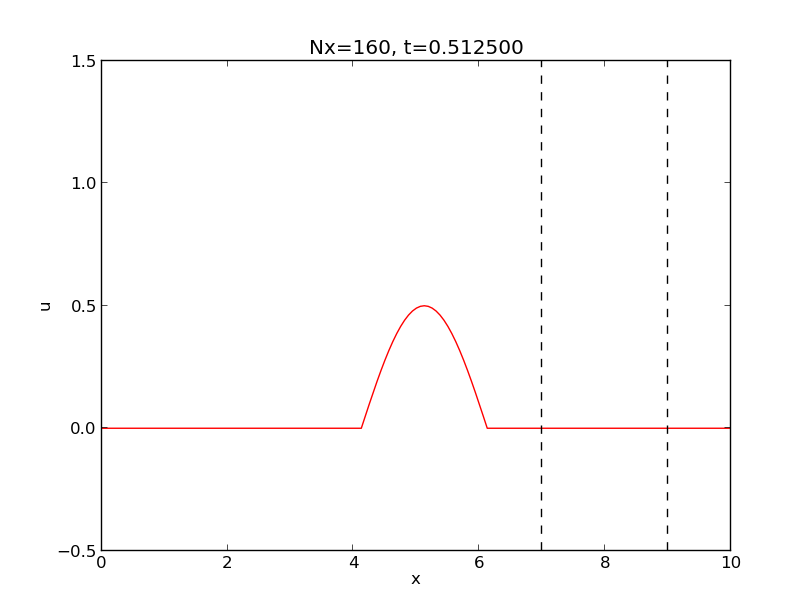
\includegraphics[width=0.9\textwidth]{../doc/src/manual/mov/wave_frames/frame_0082.png}
\newframe
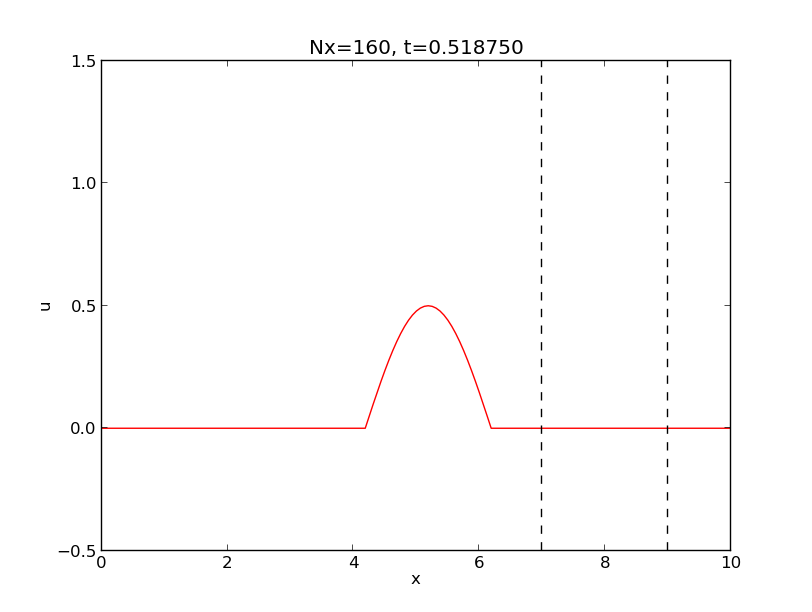
\includegraphics[width=0.9\textwidth]{../doc/src/manual/mov/wave_frames/frame_0083.png}
\newframe
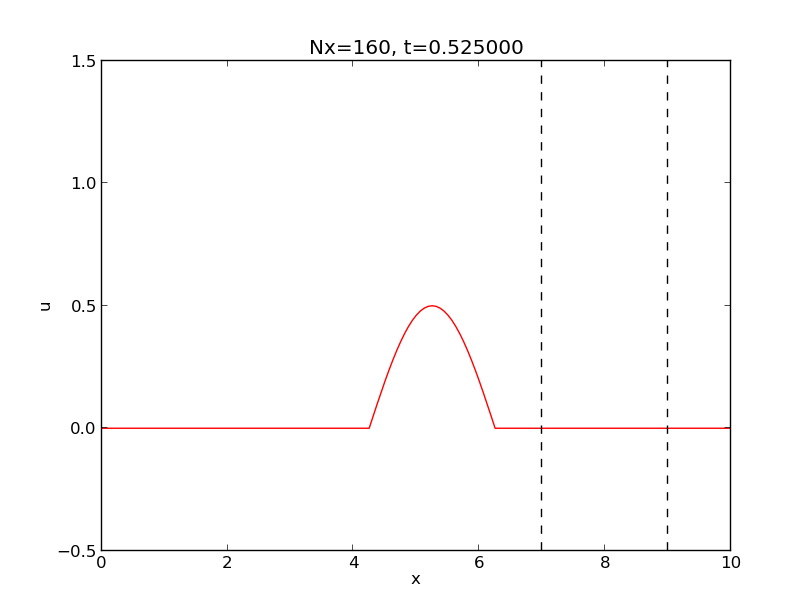
\includegraphics[width=0.9\textwidth]{../doc/src/manual/mov/wave_frames/frame_0084.png}
\newframe
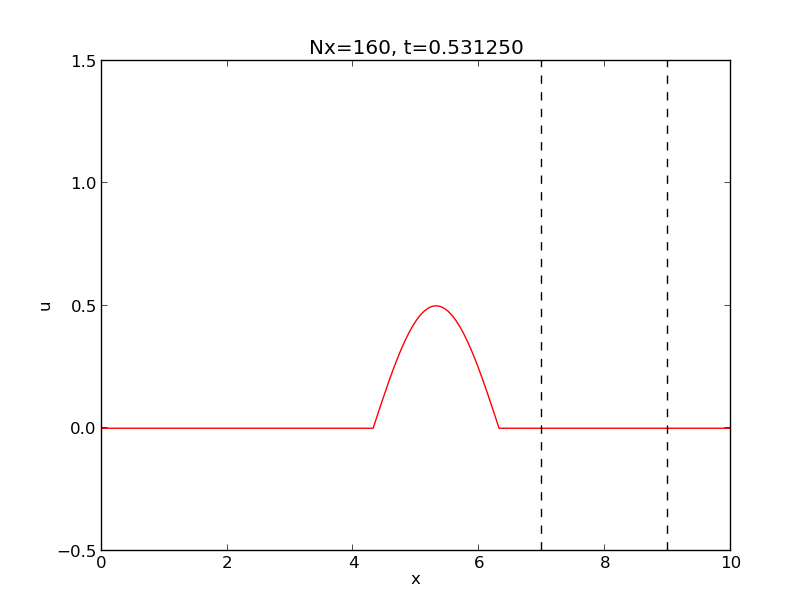
\includegraphics[width=0.9\textwidth]{../doc/src/manual/mov/wave_frames/frame_0085.png}
\newframe
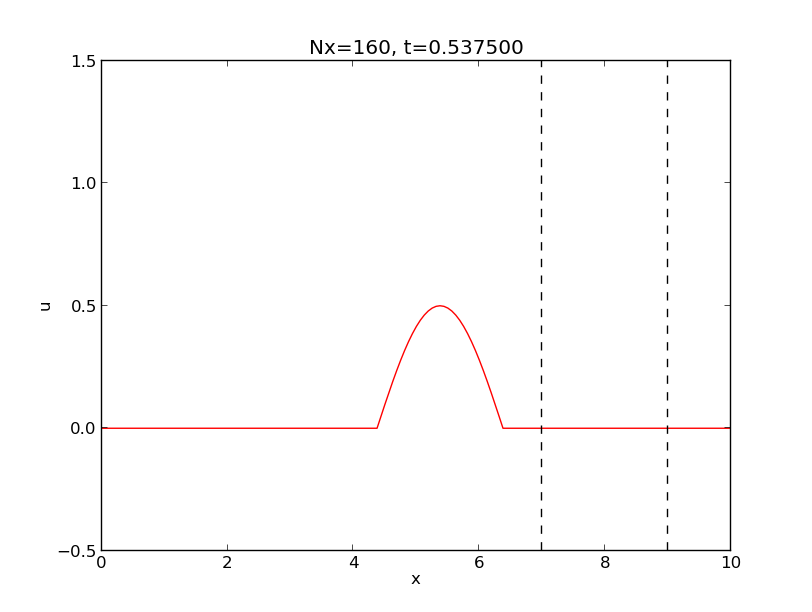
\includegraphics[width=0.9\textwidth]{../doc/src/manual/mov/wave_frames/frame_0086.png}
\newframe
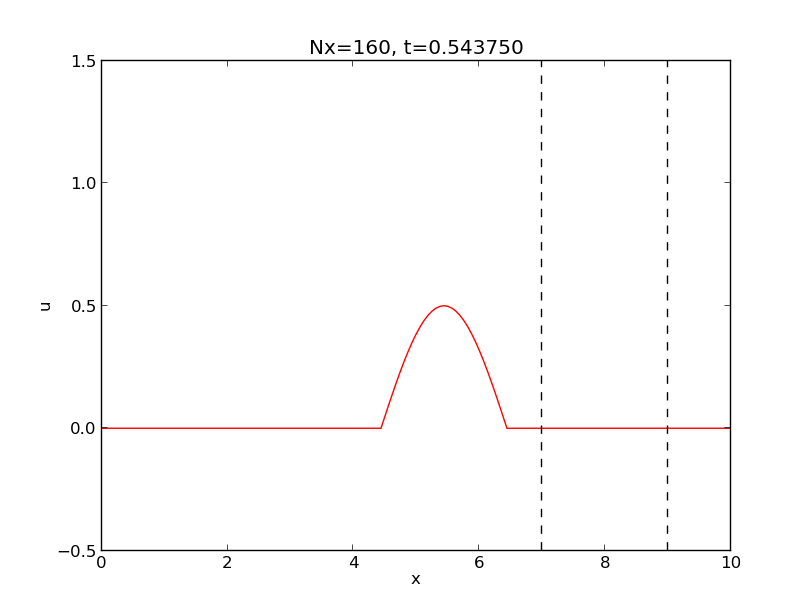
\includegraphics[width=0.9\textwidth]{../doc/src/manual/mov/wave_frames/frame_0087.png}
\newframe
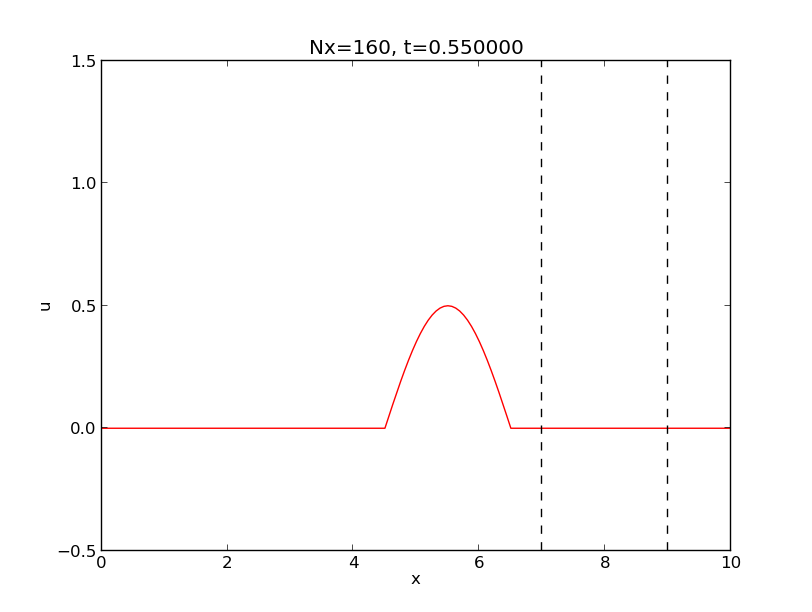
\includegraphics[width=0.9\textwidth]{../doc/src/manual/mov/wave_frames/frame_0088.png}
\newframe
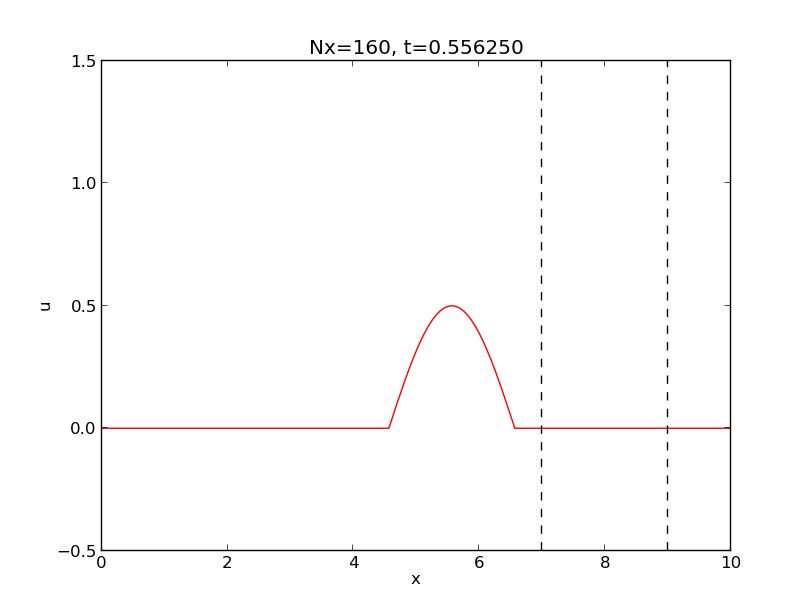
\includegraphics[width=0.9\textwidth]{../doc/src/manual/mov/wave_frames/frame_0089.png}
\newframe
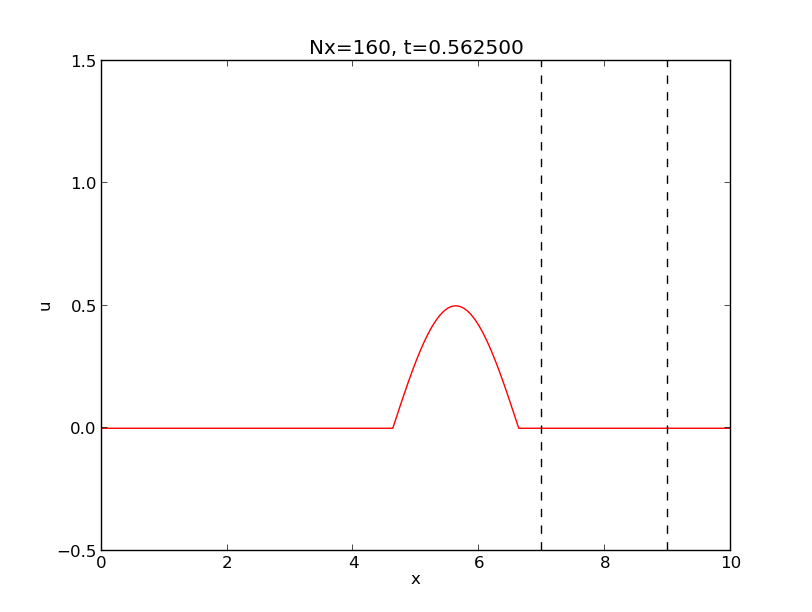
\includegraphics[width=0.9\textwidth]{../doc/src/manual/mov/wave_frames/frame_0090.png}
\newframe
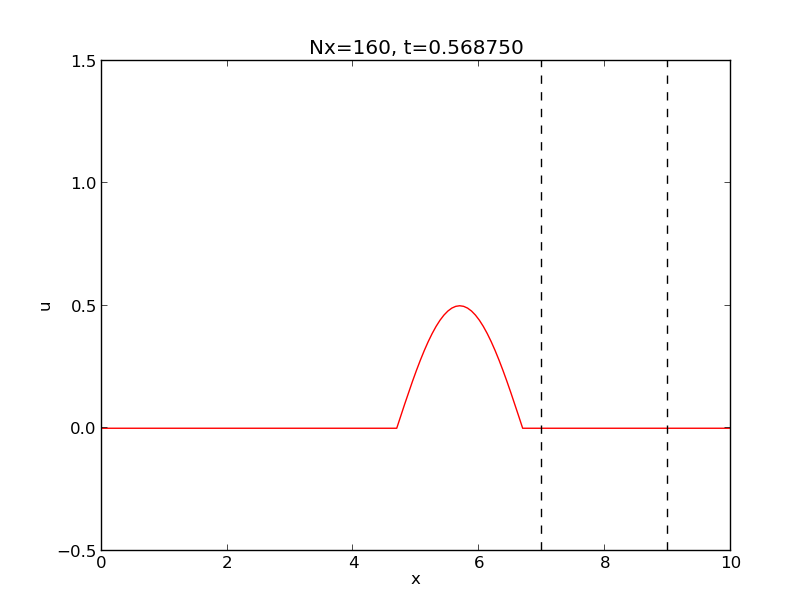
\includegraphics[width=0.9\textwidth]{../doc/src/manual/mov/wave_frames/frame_0091.png}
\newframe
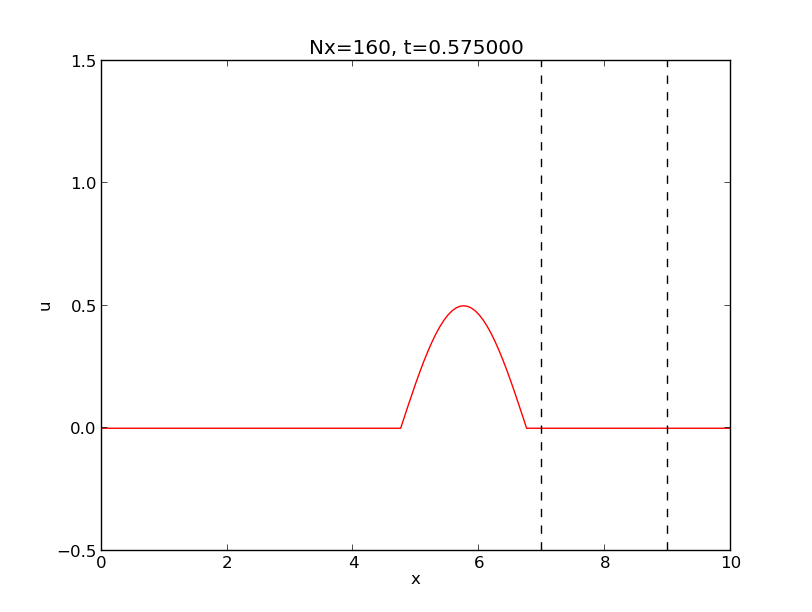
\includegraphics[width=0.9\textwidth]{../doc/src/manual/mov/wave_frames/frame_0092.png}
\newframe
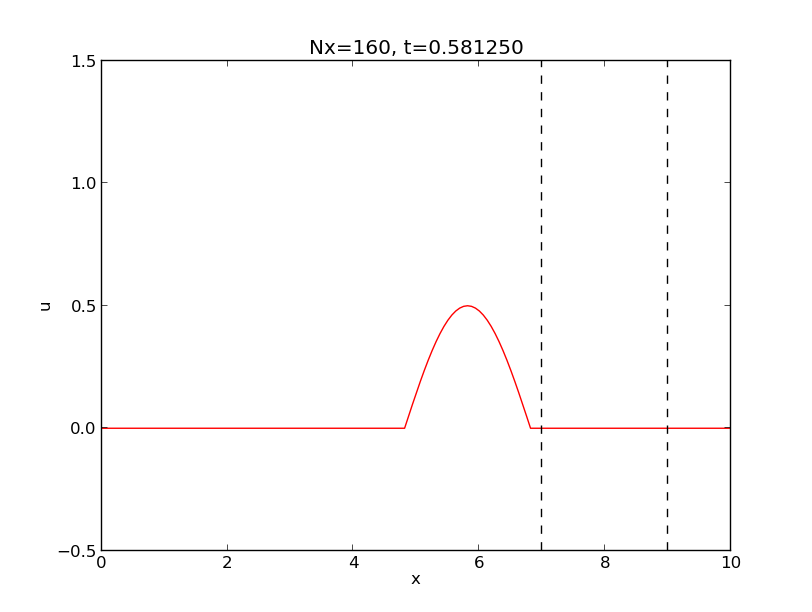
\includegraphics[width=0.9\textwidth]{../doc/src/manual/mov/wave_frames/frame_0093.png}
\newframe
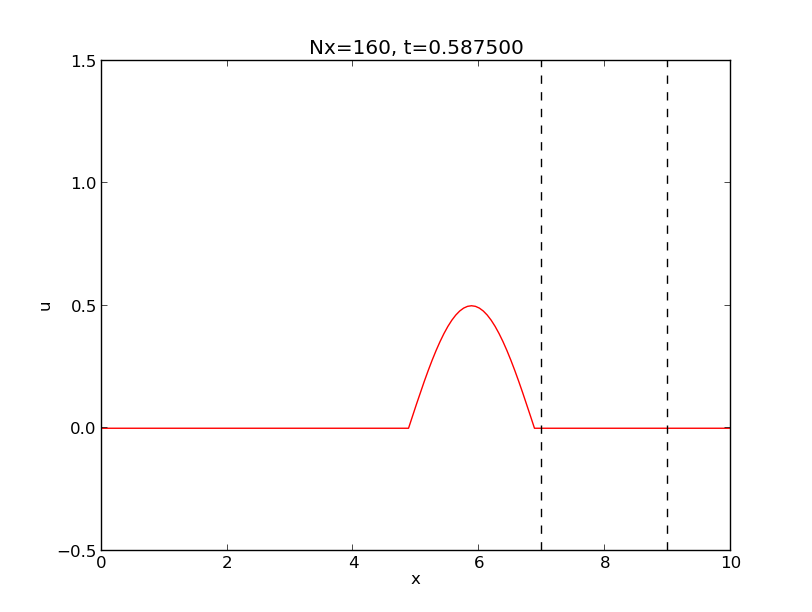
\includegraphics[width=0.9\textwidth]{../doc/src/manual/mov/wave_frames/frame_0094.png}
\newframe
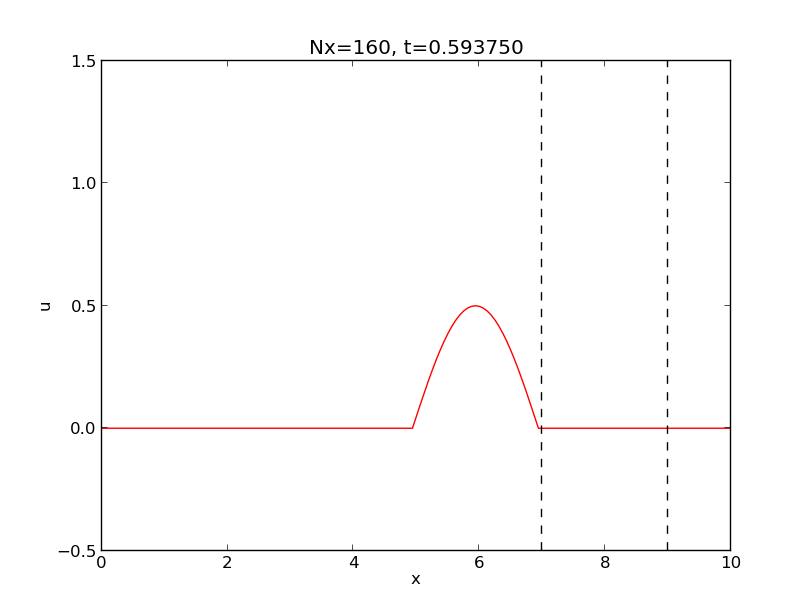
\includegraphics[width=0.9\textwidth]{../doc/src/manual/mov/wave_frames/frame_0095.png}
\newframe
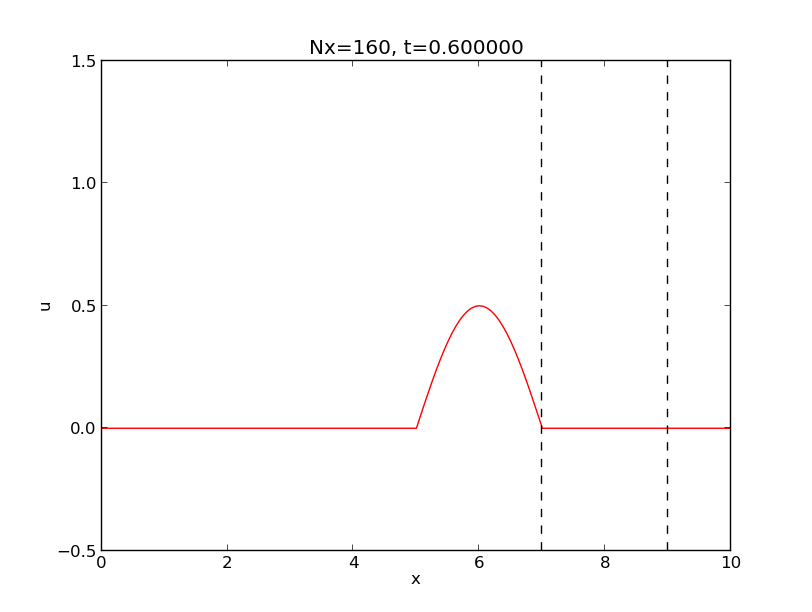
\includegraphics[width=0.9\textwidth]{../doc/src/manual/mov/wave_frames/frame_0096.png}
\newframe
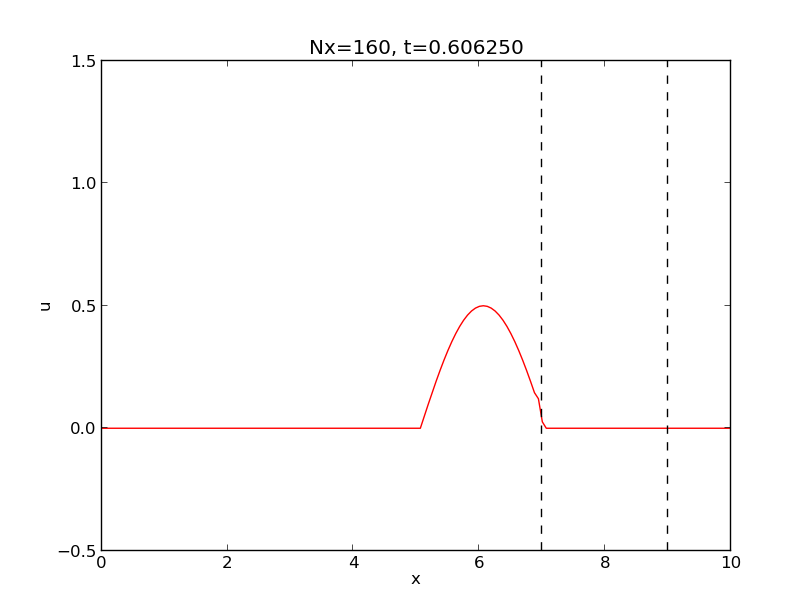
\includegraphics[width=0.9\textwidth]{../doc/src/manual/mov/wave_frames/frame_0097.png}
\newframe
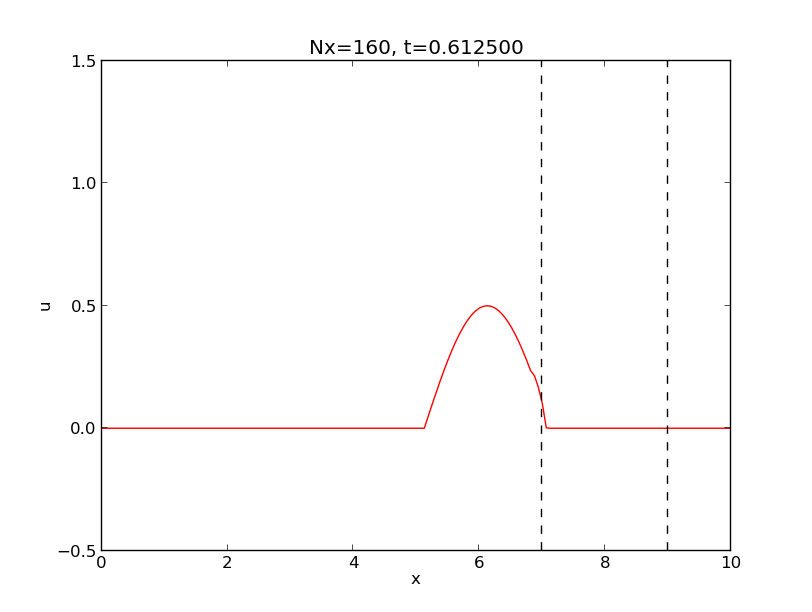
\includegraphics[width=0.9\textwidth]{../doc/src/manual/mov/wave_frames/frame_0098.png}
\newframe
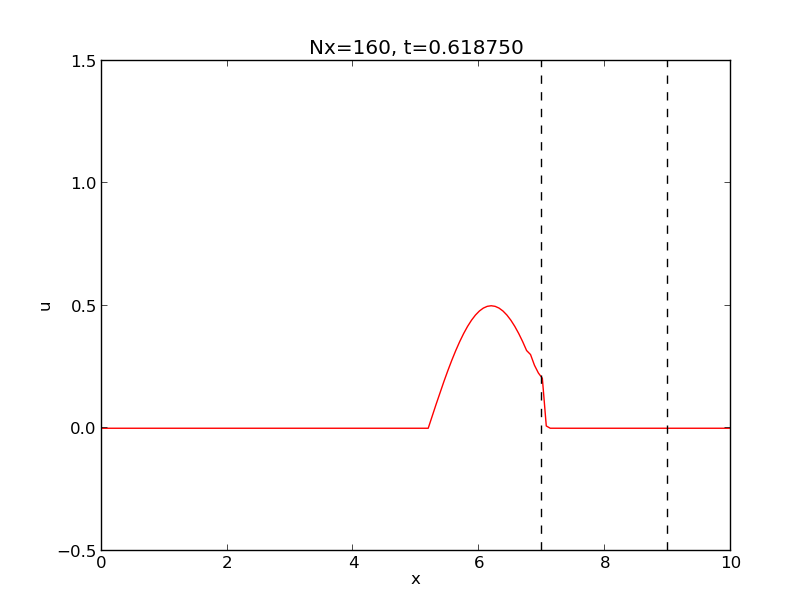
\includegraphics[width=0.9\textwidth]{../doc/src/manual/mov/wave_frames/frame_0099.png}
\newframe
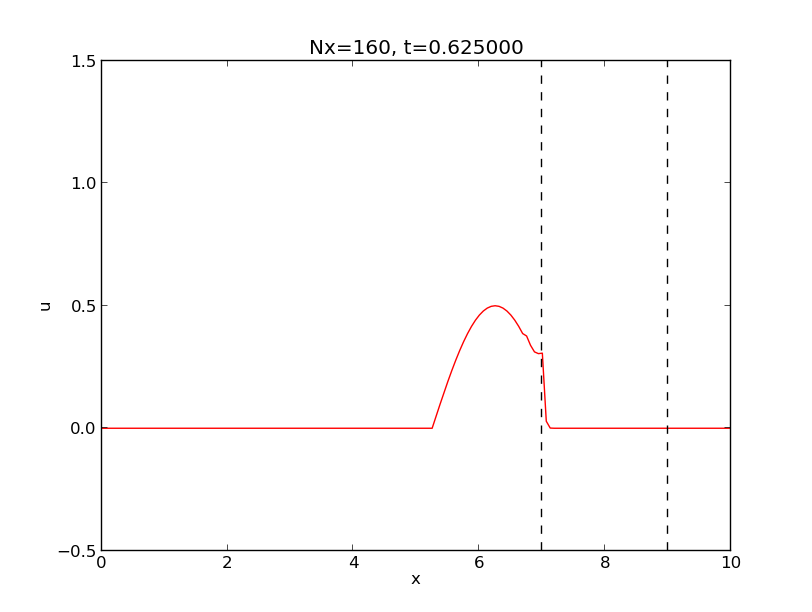
\includegraphics[width=0.9\textwidth]{../doc/src/manual/mov/wave_frames/frame_0100.png}
\newframe
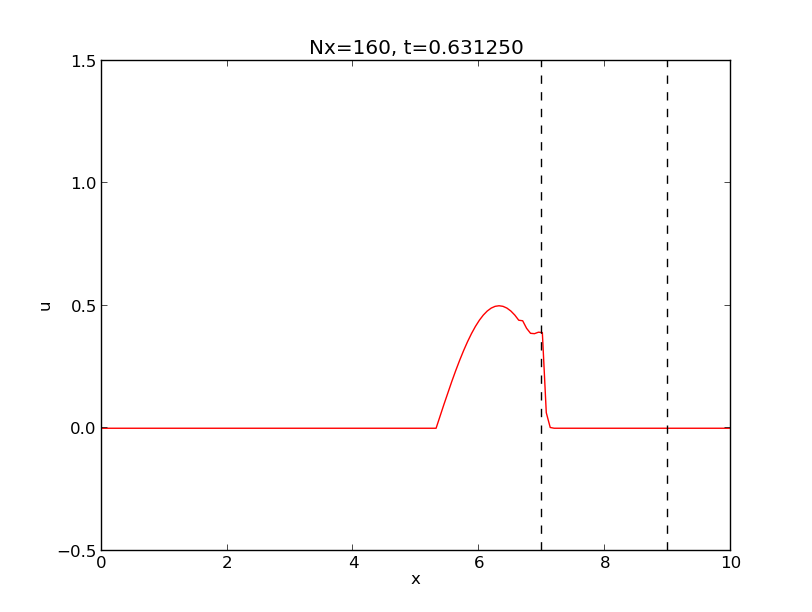
\includegraphics[width=0.9\textwidth]{../doc/src/manual/mov/wave_frames/frame_0101.png}
\newframe
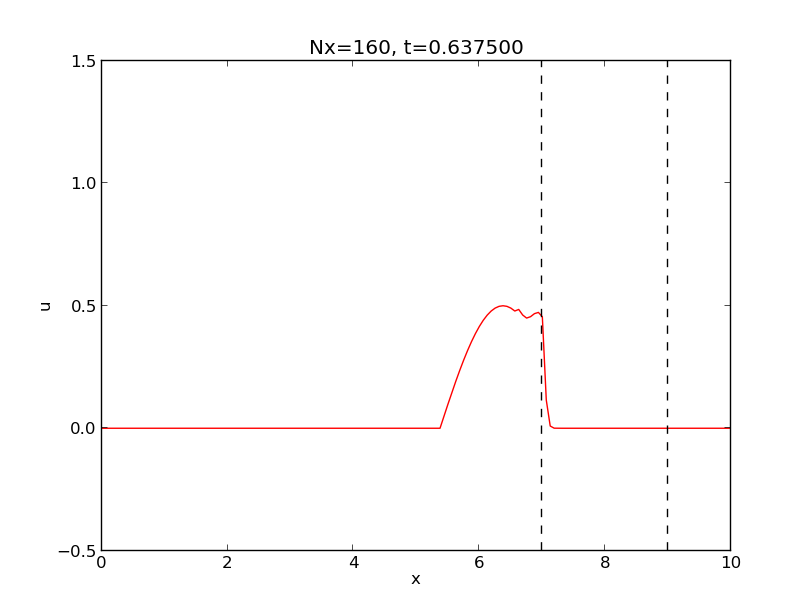
\includegraphics[width=0.9\textwidth]{../doc/src/manual/mov/wave_frames/frame_0102.png}
\newframe
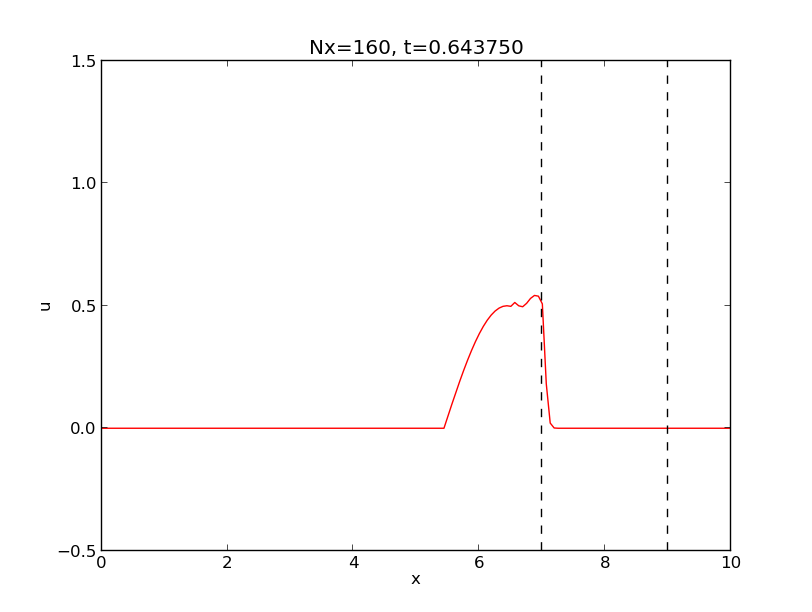
\includegraphics[width=0.9\textwidth]{../doc/src/manual/mov/wave_frames/frame_0103.png}
\newframe
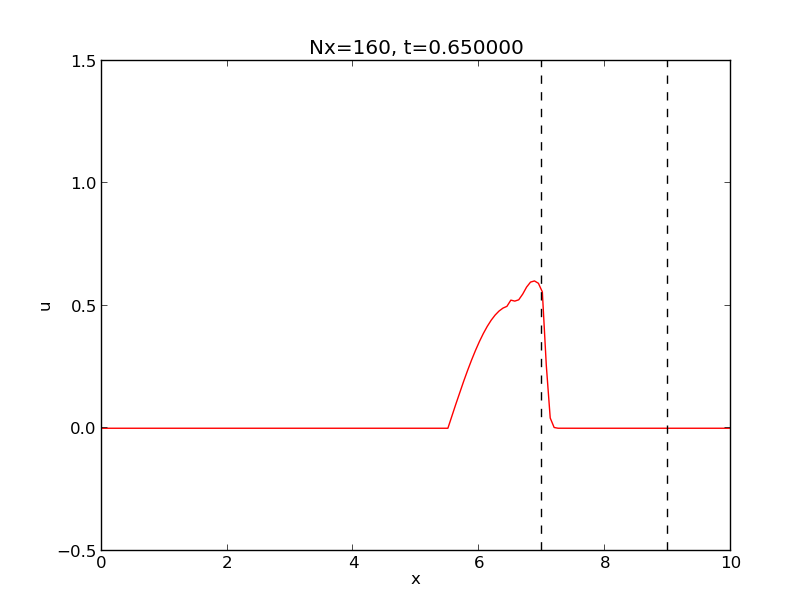
\includegraphics[width=0.9\textwidth]{../doc/src/manual/mov/wave_frames/frame_0104.png}
\newframe
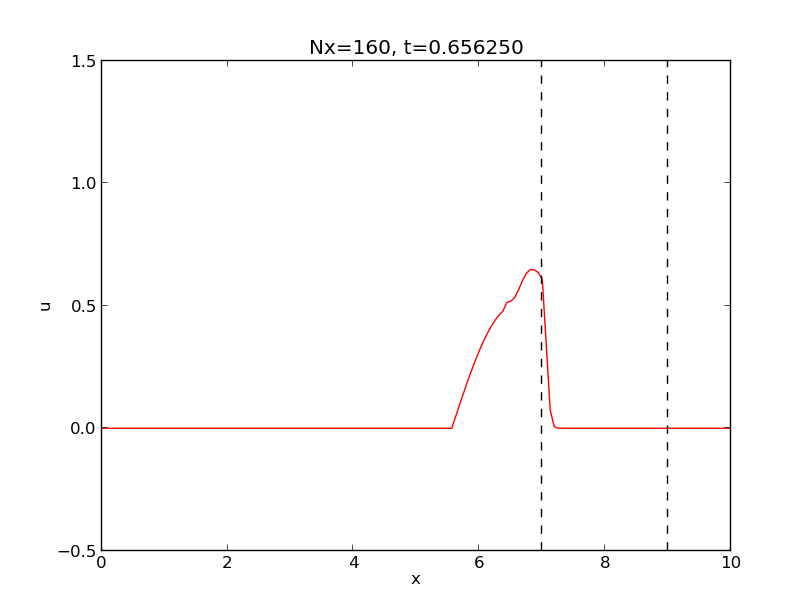
\includegraphics[width=0.9\textwidth]{../doc/src/manual/mov/wave_frames/frame_0105.png}
\newframe
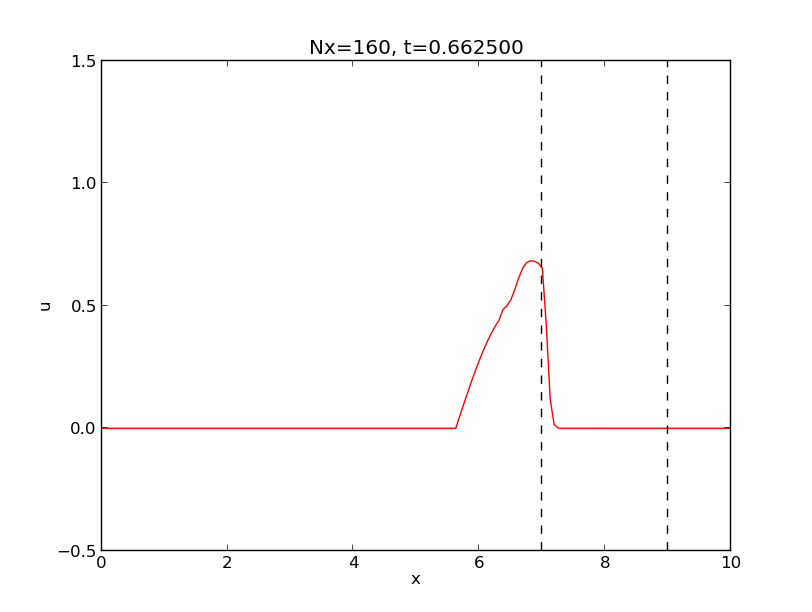
\includegraphics[width=0.9\textwidth]{../doc/src/manual/mov/wave_frames/frame_0106.png}
\newframe
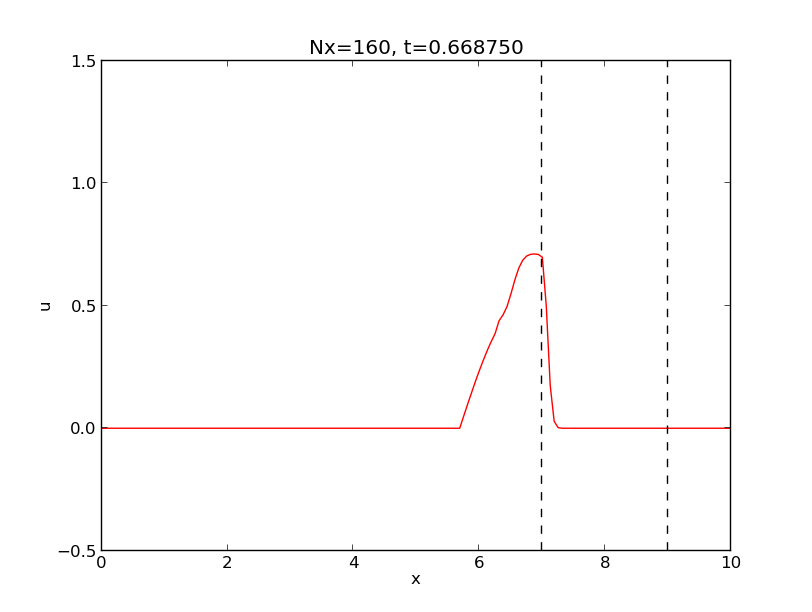
\includegraphics[width=0.9\textwidth]{../doc/src/manual/mov/wave_frames/frame_0107.png}
\newframe
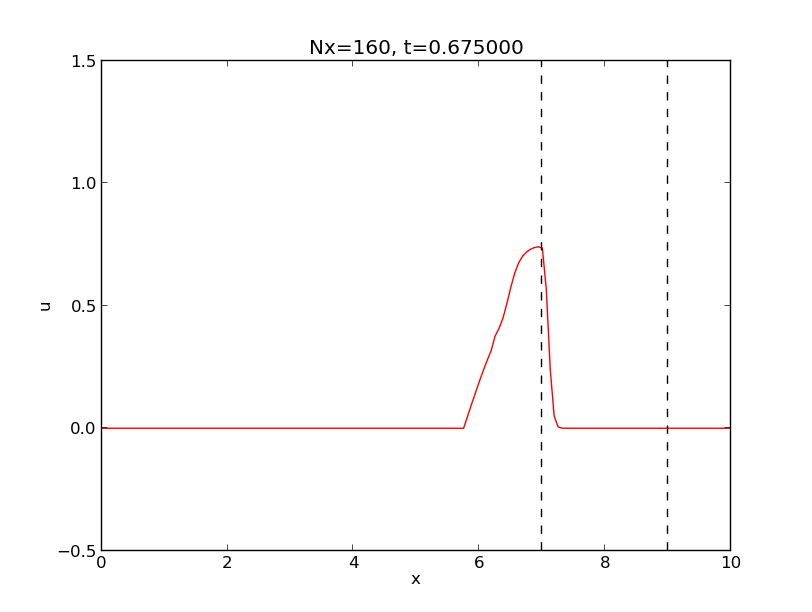
\includegraphics[width=0.9\textwidth]{../doc/src/manual/mov/wave_frames/frame_0108.png}
\newframe
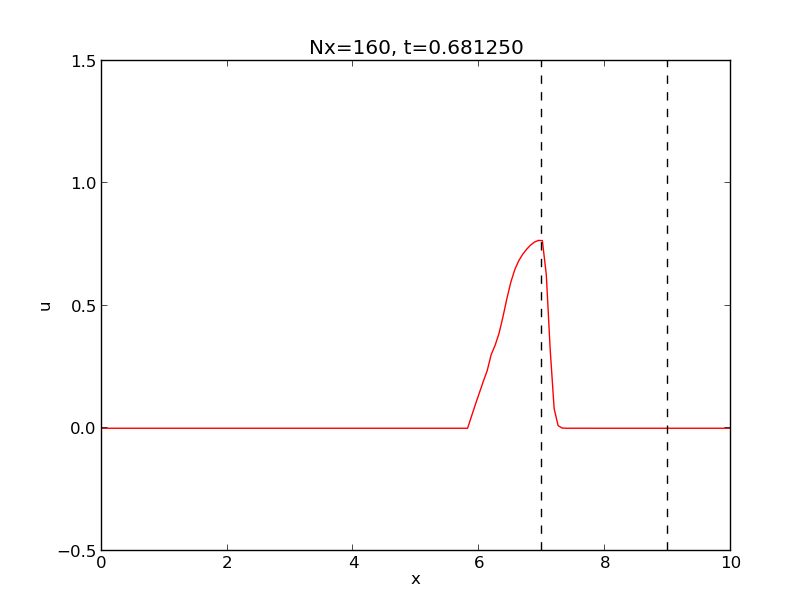
\includegraphics[width=0.9\textwidth]{../doc/src/manual/mov/wave_frames/frame_0109.png}
\newframe
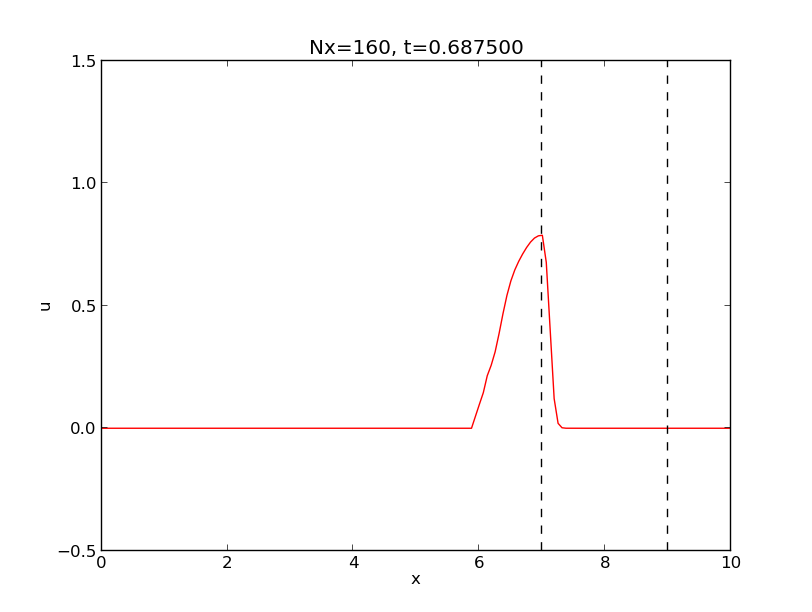
\includegraphics[width=0.9\textwidth]{../doc/src/manual/mov/wave_frames/frame_0110.png}
\newframe
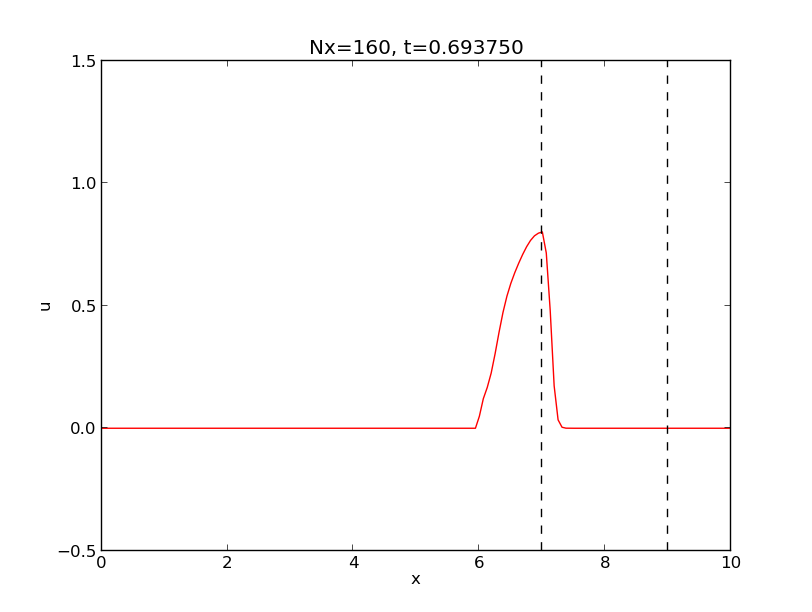
\includegraphics[width=0.9\textwidth]{../doc/src/manual/mov/wave_frames/frame_0111.png}
\newframe
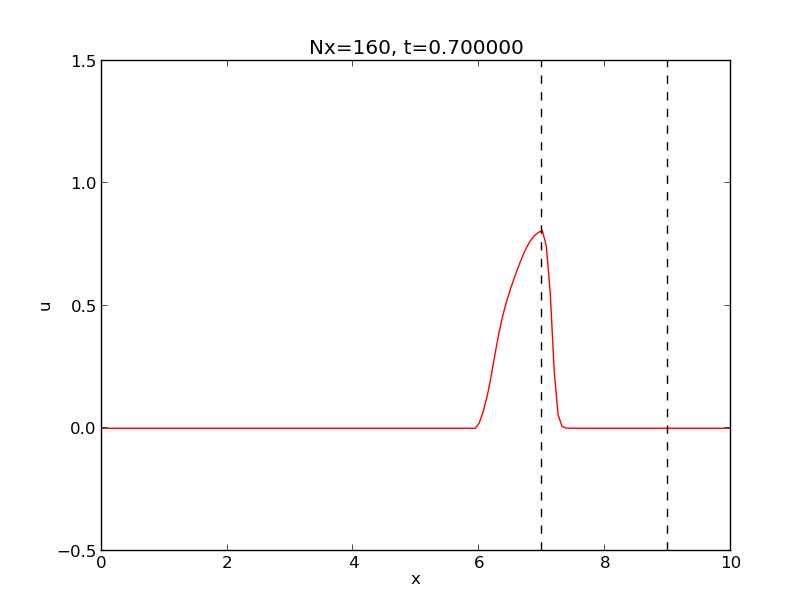
\includegraphics[width=0.9\textwidth]{../doc/src/manual/mov/wave_frames/frame_0112.png}
\newframe
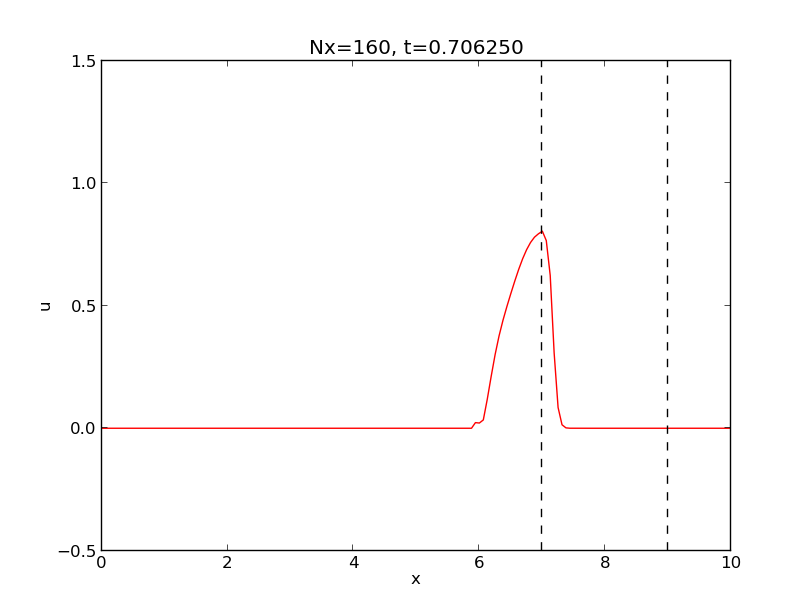
\includegraphics[width=0.9\textwidth]{../doc/src/manual/mov/wave_frames/frame_0113.png}
\newframe
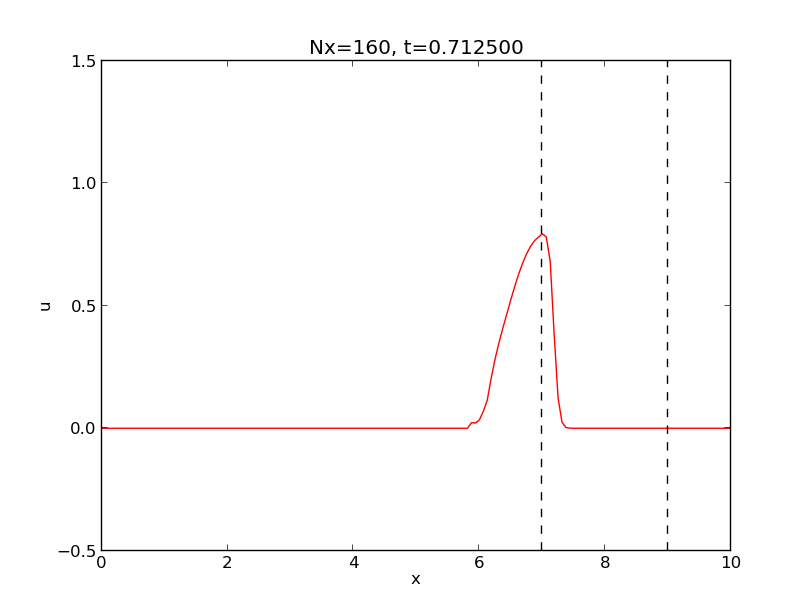
\includegraphics[width=0.9\textwidth]{../doc/src/manual/mov/wave_frames/frame_0114.png}
\newframe
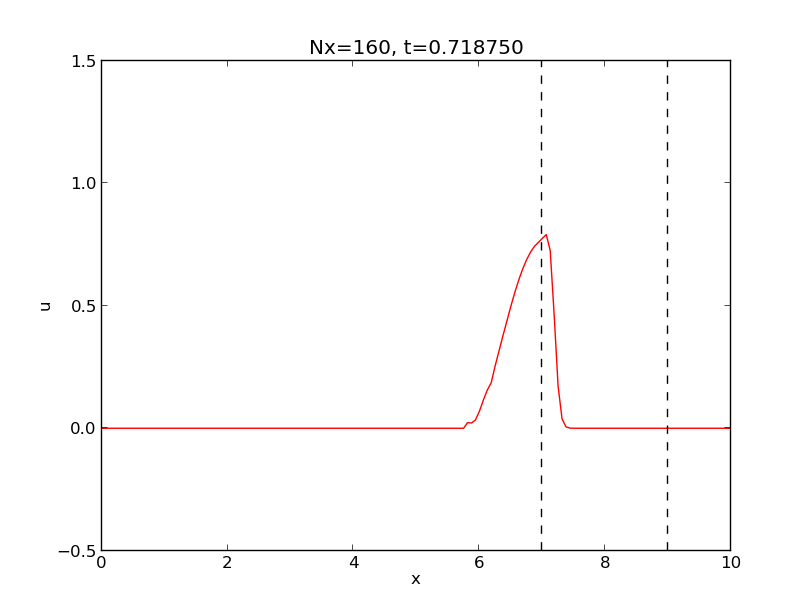
\includegraphics[width=0.9\textwidth]{../doc/src/manual/mov/wave_frames/frame_0115.png}
\newframe
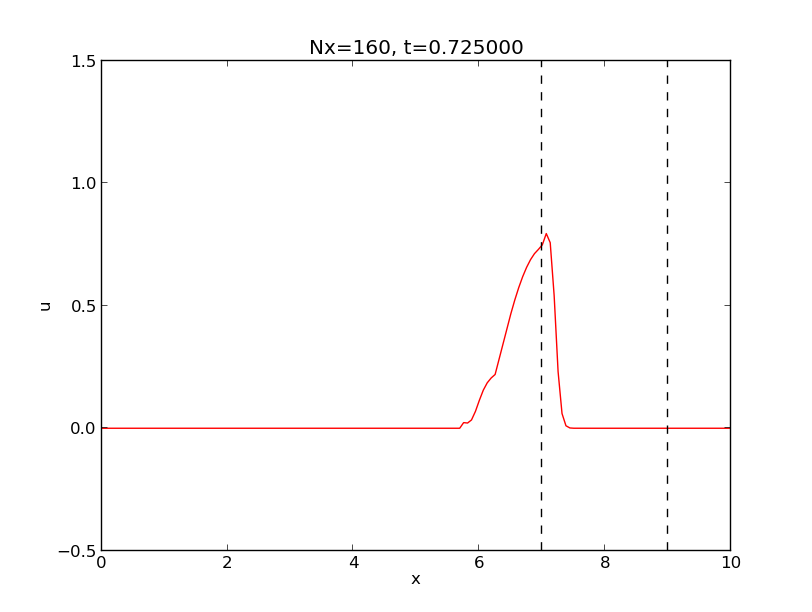
\includegraphics[width=0.9\textwidth]{../doc/src/manual/mov/wave_frames/frame_0116.png}
\newframe
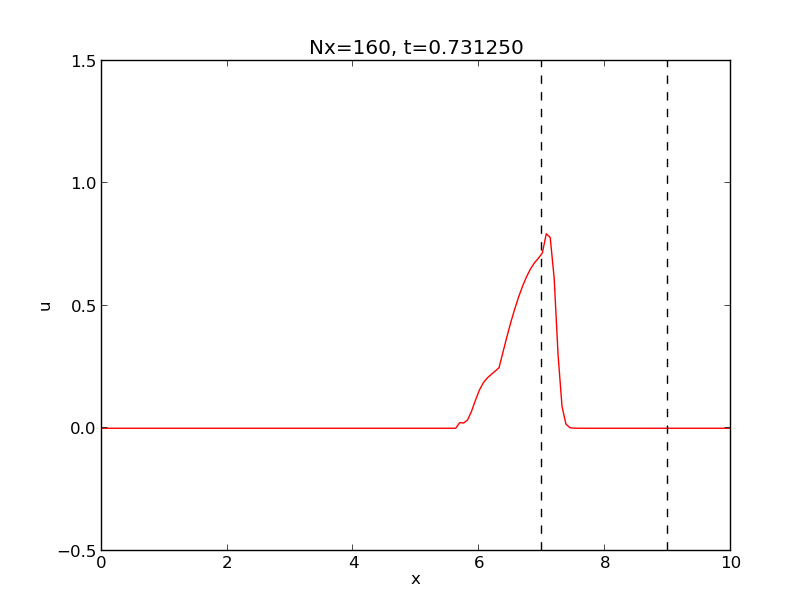
\includegraphics[width=0.9\textwidth]{../doc/src/manual/mov/wave_frames/frame_0117.png}
\newframe
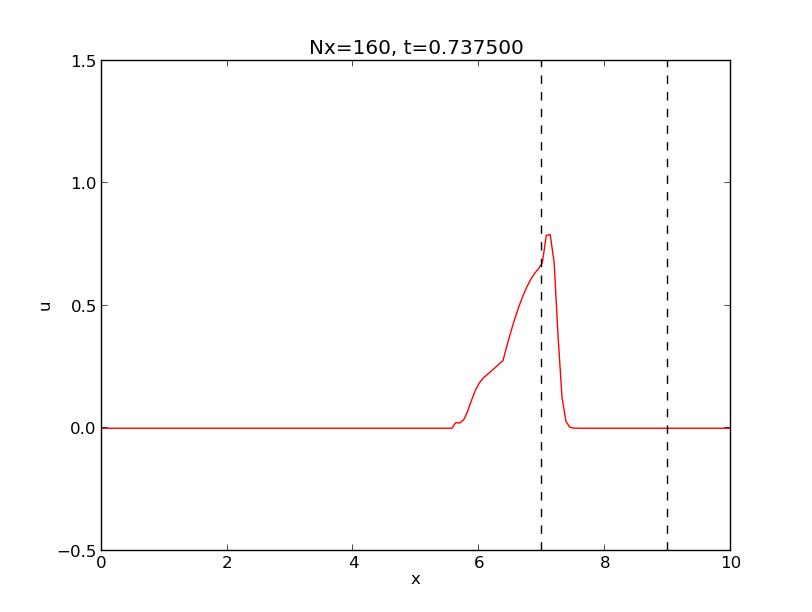
\includegraphics[width=0.9\textwidth]{../doc/src/manual/mov/wave_frames/frame_0118.png}
\newframe
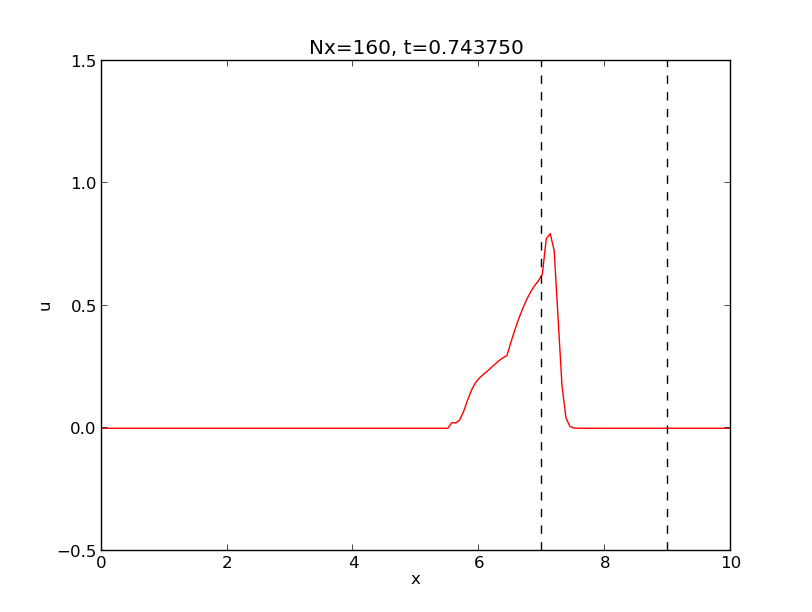
\includegraphics[width=0.9\textwidth]{../doc/src/manual/mov/wave_frames/frame_0119.png}
\newframe
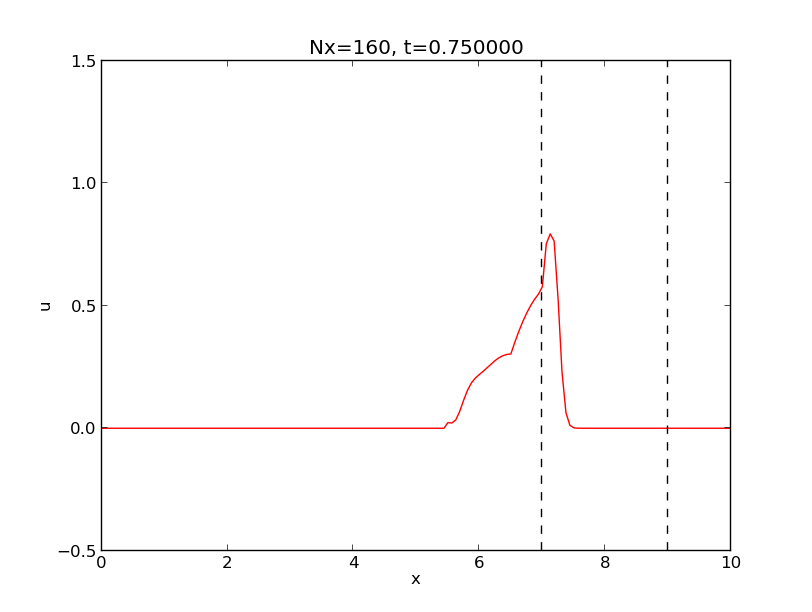
\includegraphics[width=0.9\textwidth]{../doc/src/manual/mov/wave_frames/frame_0120.png}
\newframe
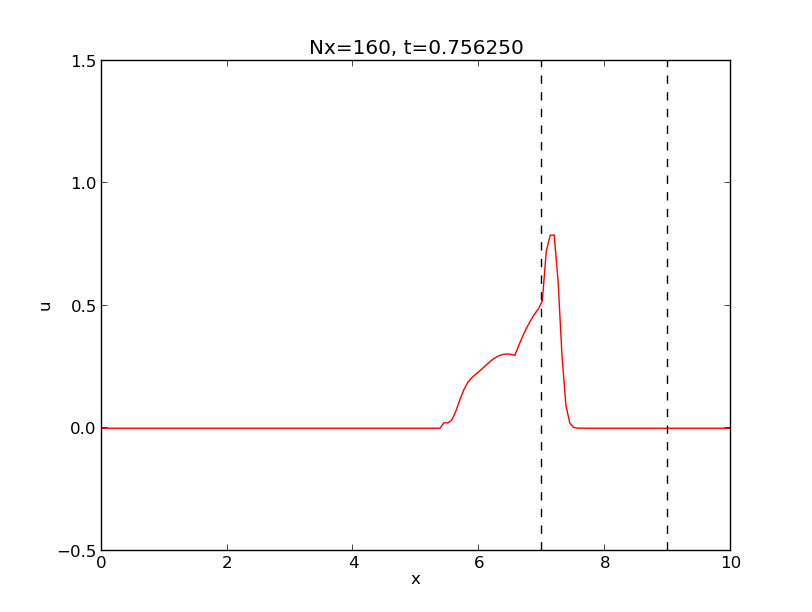
\includegraphics[width=0.9\textwidth]{../doc/src/manual/mov/wave_frames/frame_0121.png}
\newframe
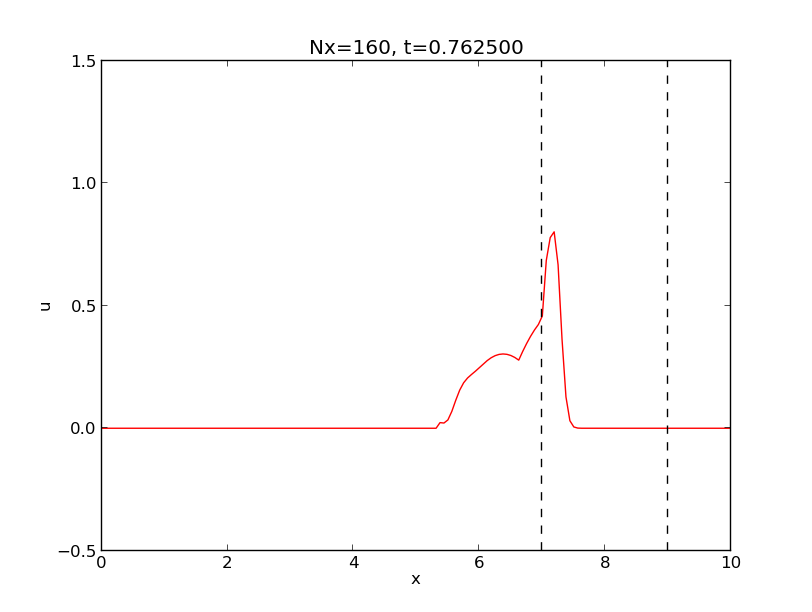
\includegraphics[width=0.9\textwidth]{../doc/src/manual/mov/wave_frames/frame_0122.png}
\newframe
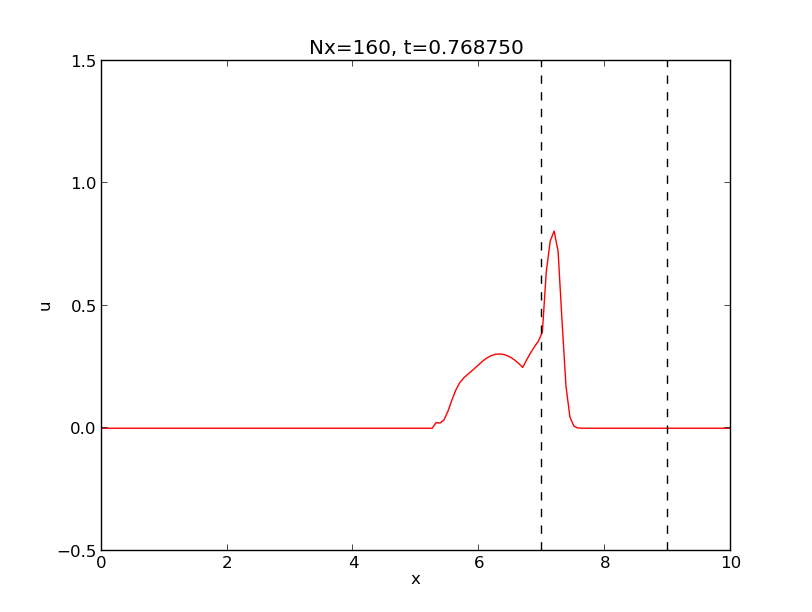
\includegraphics[width=0.9\textwidth]{../doc/src/manual/mov/wave_frames/frame_0123.png}
\newframe
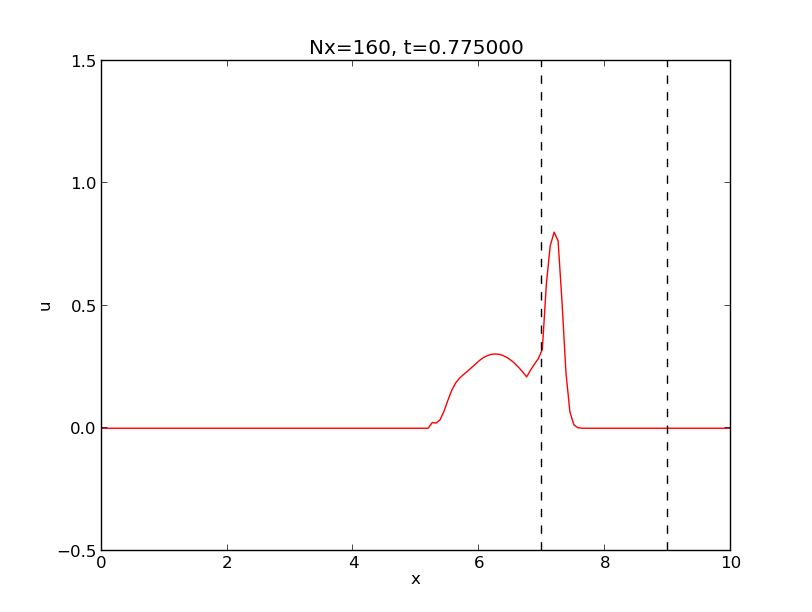
\includegraphics[width=0.9\textwidth]{../doc/src/manual/mov/wave_frames/frame_0124.png}
\newframe
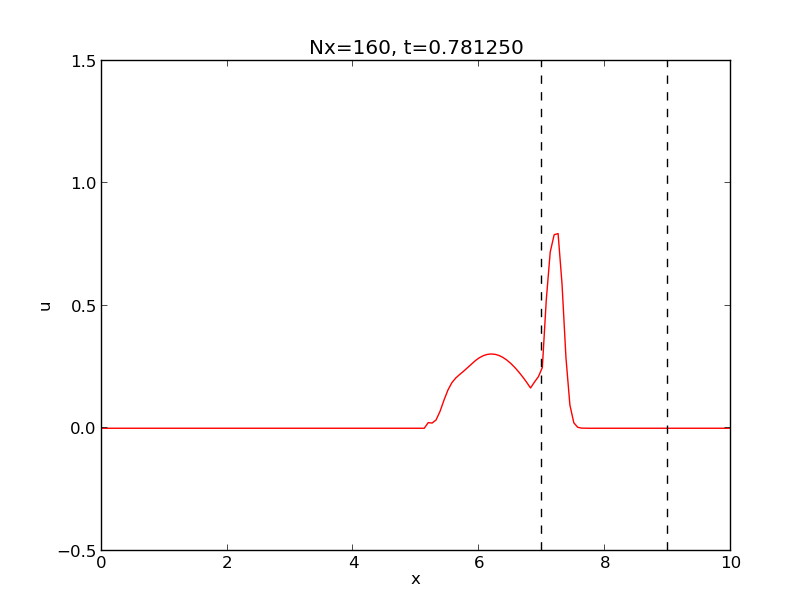
\includegraphics[width=0.9\textwidth]{../doc/src/manual/mov/wave_frames/frame_0125.png}
\newframe
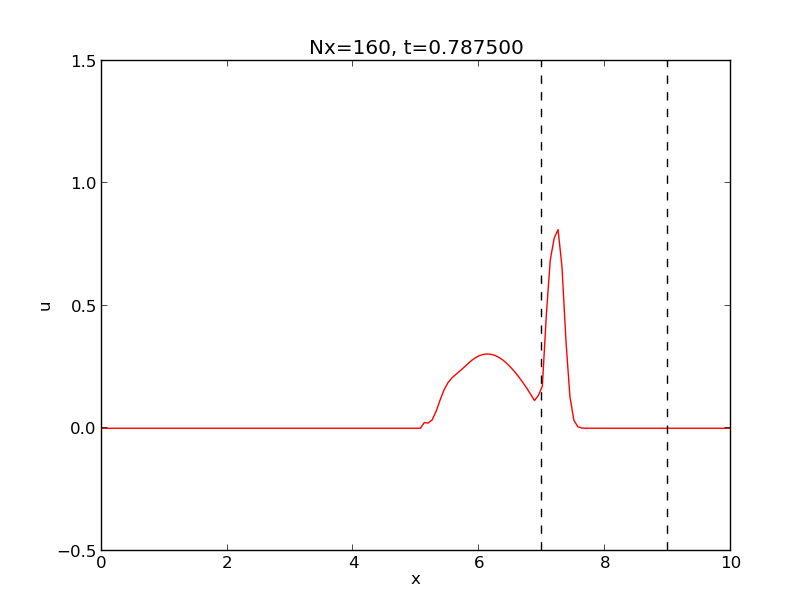
\includegraphics[width=0.9\textwidth]{../doc/src/manual/mov/wave_frames/frame_0126.png}
\newframe
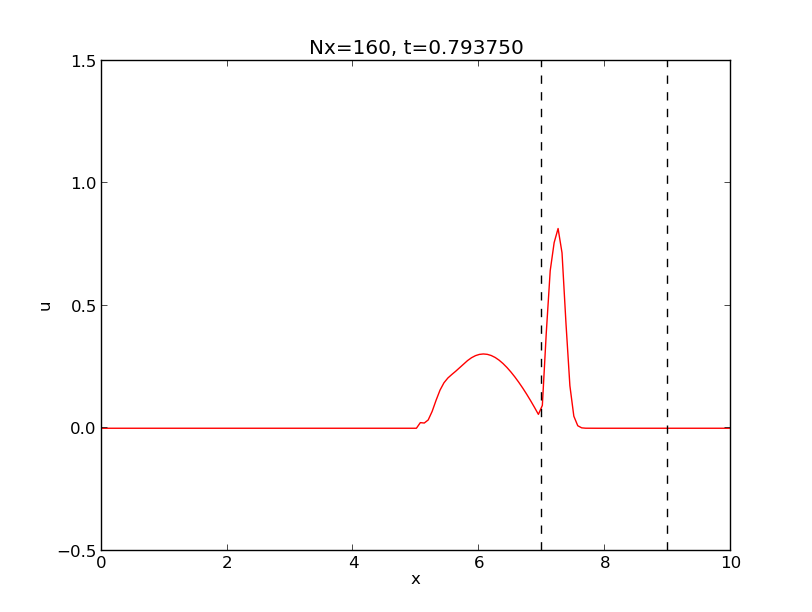
\includegraphics[width=0.9\textwidth]{../doc/src/manual/mov/wave_frames/frame_0127.png}
\newframe
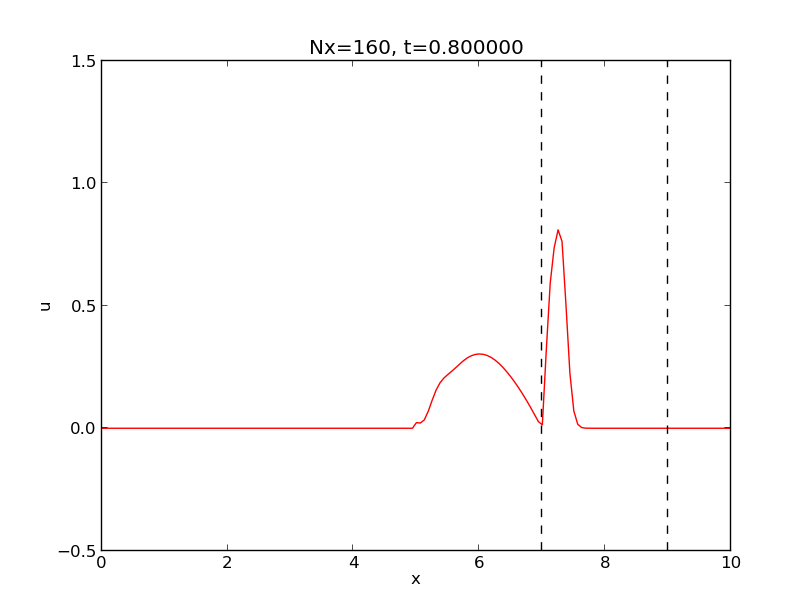
\includegraphics[width=0.9\textwidth]{../doc/src/manual/mov/wave_frames/frame_0128.png}
\newframe
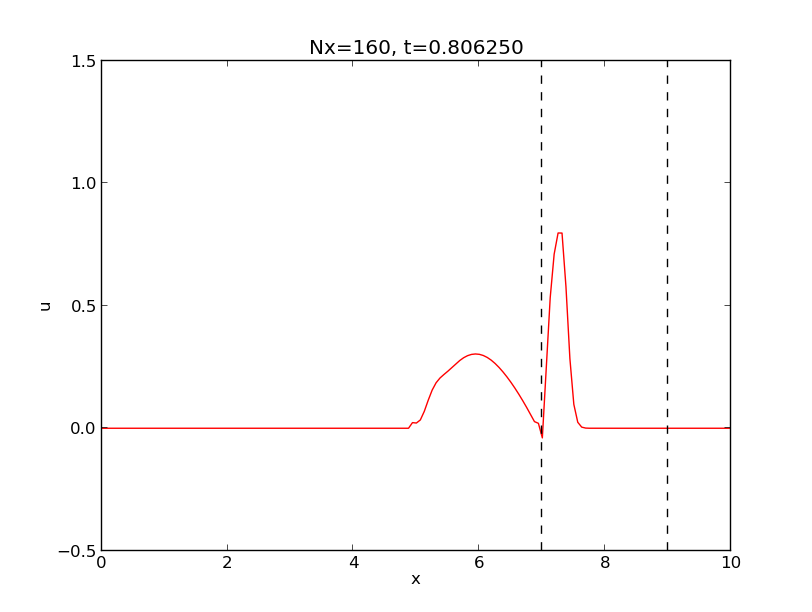
\includegraphics[width=0.9\textwidth]{../doc/src/manual/mov/wave_frames/frame_0129.png}
\end{animateinline}
\end{center}

\begin{center}  % movie caption
Movie \arabic{doconce:movie:counter}: Animated collection of images.
\end{center}
\end{doconce:movie}


Here is the same collection, but with images in cyberspace, given as URLs:



\begin{Verbatim}[numbers=none,fontsize=\fontsize{9pt}{9pt},baselinestretch=0.95]
https://hplgit.github.io/animate/..../frame_%04d.png:80->129

\end{Verbatim}



\begin{doconce:movie}
\refstepcounter{doconce:movie:counter}
\begin{center}
Taking images to animate from cyberspace. \Verb!https://hplgit.github.io/animate/doc/pub/mov-animate/frames/frame_%04d.png:80->129!: load \href{{file:///X/X/movie_player1.html}}{\nolinkurl{movie_player1.html}} into a browser
\end{center}

\begin{center}  % movie caption
Movie \arabic{doconce:movie:counter}: Taking images to animate from cyberspace.
\end{center}
\end{doconce:movie}


The movie above in MPEG format, typeset in a box:


\begin{center}
\begin{Sbox}
\begin{minipage}{0.85\linewidth}

\begin{doconce:movie}
\refstepcounter{doconce:movie:counter}
\begin{center}
% movie15 package
\includemovie[poster,
label=docsrcmanualmovwavempeg,
autoplay,
controls,
toolbar,
text={\small (Loading ../doc/src/manual/mov/wave.mpeg)},
repeat,
]{0.9\linewidth}{0.9\linewidth}{../doc/src/manual/mov/wave.mpeg}

\movieref[rate=0.5]{docsrcmanualmovwavempeg}{Slower}
\movieref[rate=2]{docsrcmanualmovwavempeg}{Faster}
\movieref[default]{docsrcmanualmovwavempeg}{Normal}
\movieref[pause]{docsrcmanualmovwavempeg}{Play/Pause}
\movieref[stop]{docsrcmanualmovwavempeg}{Stop}
\end{center}

\begin{center}  % movie caption
Movie \arabic{doconce:movie:counter}: 1D wave in MPEG. \label{mov:wave}
\end{center}
\end{doconce:movie}
\end{minipage}
\end{Sbox}
\fbox{\TheSbox}
\end{center}

Here is the same movie in AVI format:


\begin{doconce:movie}
\refstepcounter{doconce:movie:counter}
\begin{center}
% movie15 package
\includemovie[poster,
label=docsrcmanualmovwaveavi,
autoplay,
controls,
toolbar,
text={\small (Loading ../doc/src/manual/mov/wave.avi)},
repeat,
]{0.9\linewidth}{0.9\linewidth}{../doc/src/manual/mov/wave.avi}

\movieref[rate=0.5]{docsrcmanualmovwaveavi}{Slower}
\movieref[rate=2]{docsrcmanualmovwaveavi}{Faster}
\movieref[default]{docsrcmanualmovwaveavi}{Normal}
\movieref[pause]{docsrcmanualmovwaveavi}{Play/Pause}
\movieref[stop]{docsrcmanualmovwaveavi}{Stop}
\end{center}

\begin{center}  % movie caption
Movie \arabic{doconce:movie:counter}: 1D wave in AVI.
\end{center}
\end{doconce:movie}


Here is the same movie, but with a URL to GitHub:


\begin{doconce:movie}
\refstepcounter{doconce:movie:counter}
\begin{quote}
% link to web movie
Movie \arabic{doconce:movie:counter}:  \href{https://hplgit.github.io/animate/doc/pub/mov-animate/demo.ogg}{\nolinkurl{https://hplgit.github.io/animate/doc/pub/mov-animate/demo.ogg}}
\end{quote}
\end{doconce:movie}


Here is a YouTube video:


\begin{doconce:movie}
\refstepcounter{doconce:movie:counter}
\begin{center}
\includemedia[
width=0.6\linewidth,height=0.45\linewidth,
activate=pageopen,
flashvars={
modestbranding=1   % no YouTube logo in control bar
&autohide=1        % controlbar autohide
&showinfo=0        % no title and other info before start
&rel=0             % no related videos after end
},
]{}{https://www.youtube.com/watch?v=_O7iUiftbKU}
\end{center}

\begin{center}  % movie caption
Movie \arabic{doconce:movie:counter}: YouTube movie.
\end{center}
\end{doconce:movie}


And a vimeo video:


\begin{doconce:movie}
\refstepcounter{doconce:movie:counter}
\begin{center}\href{{https://vimeo.com/55562330}}{\nolinkurl{https://vimeo.com/55562330}}\end{center}

\begin{center}  % movie caption
Movie \arabic{doconce:movie:counter}: Vimeo movie.
\end{center}
\end{doconce:movie}


Finally, let us demonstrate referencing the movie~\ref{mov:wave}.

% ------------------- end of main content ---------------

\end{document}

